\label{tab}
%Insérer dans le préambule :

 \maboite{\BS{usepackage}\AC{tkz-tab}}


%\subsection{Déclaration du tableau}
\SbSSCT{Déclaration du tableau}{Creation of the table}

\begin{tabular}{|l|c|}\hline 
\begin{tikzpicture}
\tkzTabInit{1° ligne / 1 ,2° ligne /1 }{ a , b, c }
%\tkzTabLine{ 1, 2, 3 , 4,5 }
\end{tikzpicture}
\\ \hline 
\BS{begin}\AC{tikzpicture} \\
\BSS{tkzTabInit}\AC{1° ligne / 1 ,2° ligne /1 } \AC{ a , b, c } \\
% \BSS{tkzTabLine}\AC{ 1, 2, 3 , 4,5 } \\
\BS{end}\AC{tikzpicture}
 \\ \hline 
 \end{tabular} 

\subsubsection{Options}
 
%\paragraph{Hauteur des lignes}:

\begin{tabular}{|l|c|}\hline  
 \multicolumn{1}{|c|}{\textbf{\TFRGB{Hauteur des ligne}{Row width }} }
 \\ \hline


\begin{tikzpicture} \tkzTabInit{1° ligne /1  , 2° ligne /.5  , 3° ligne /1.5 }{a , b , c }\end{tikzpicture}
\\ \hline 
\BS{tikz}  \BSS{tkzTabInit}\AC{1° ligne {'\color{red}  /1}  , 2° ligne {\color{red}   /.5}  , 3° ligne {\color{red}  /1.5} }\AC{a , b , c };
\\ \hline 
\end{tabular} 
 
\bigskip
%\paragraph{Largeur de la première colonne } :

\begin{tabular}{|l|c|}\hline 
 \multicolumn{1}{|c|}{\textbf{\TFRGB{Largeur de la première colonne  }{First column width }} }
 \\ \hline
\begin{tikzpicture} 
\tkzTabInit[lgt=4]{ $x$ / 1}{ a , b , c  }
\end{tikzpicture}
\\ \hline 
\BS{tkzTabInit}[\RDD{lgt}=4]\AC{ $x$ / 1}\AC{ a , b , c  }; \\
\dft :  lgt==2 cm 
\\ \hline 
\end{tabular} 

\bigskip

%\paragraph{Espacement entre deux valeurs} :
%\Par{Espacement entre deux valeurs}{Space between two values} :


\begin{tabular}{|l|c|}\hline 
 \multicolumn{1}{|c|}{\textbf{\TFRGB{Espacement entre deux valeurs}{Space between two values}} }
 \\ \hline

\begin{tikzpicture} 
\tkzTabInit[espcl=2]{ $x$ / 1}{ a , b , c  }
\end{tikzpicture}
\\ \hline 
\BS{tkzTabInit}[\RDD{espcl}=1]\AC{ $x$ / 1}\AC{ a , b , c  }; \\
\dft :  espcl=2 cm
\\ \hline 
\end{tabular}


\bigskip
%\paragraph{Marge de début et de fin} :

\begin{tabular}{|l|c|}\hline 
 \multicolumn{1}{|c|}{\textbf{\TFRGB{Marge de début et de fin  }{Margin  }} }
 \\ \hline
\begin{tikzpicture} 
\tkzTabInit[deltacl=2]{ $x$ / 1}{ a , b , c  }
\end{tikzpicture} 
\\ \hline 
\BS{tkzTabInit}[\RDD{deltacl}=1]\AC{ $x$ / 1}\AC{ a , b , c  }; \\
\dft :  deltacl=0.5 cm
\\ \hline 
\end{tabular}



\newpage
%\paragraph{\'Epaisseur des lignes du tableau } : 

\begin{tabular}{|l|c|}\hline 
 \multicolumn{1}{|c|}{\textbf{\TFRGB{\'Epaisseur des lignes du tableau }{Line width }} }
 \\ \hline
\begin{tikzpicture} 
\tkzTabInit[lw=2pt]{ $x$ / 1}{ a , b , c  }
\end{tikzpicture} 
\\ \hline 
\BS{tkzTabInit}[\RDD{dlw}=2pt]\AC{ $x$ / 1}\AC{ a , b , c  }; \\
\dft :  lw=0,4 pt
\\ \hline 
\end{tabular}



\bigskip
%\paragraph{Absence de cadre} :

\begin{tabular}{|l|c|}\hline
 \multicolumn{1}{|c|}{\textbf{\TFRGB{Absence de cadre}{No cadre}} }
 \\ \hline 
\begin{tikzpicture} 
\tkzTabInit[nocadre]{ $x$ / 1}{ a , b , c  }
\end{tikzpicture} 
\\ \hline 
\BS{tkzTabInit}[nocadre]\AC{ $x$ / 1}\AC{ a , b , c  }; \\
\dft :  nocadre=false
\\ \hline 
\end{tabular}


\bigskip
%\paragraph{Mise en couleur}:\\
\begin{tabular}{|c|c|}\hline
 \multicolumn{2}{|c|}{\textbf{\TFRGB{Mise en couleur  }{ Coloring }} }
 \\ \hline 
\multicolumn{2}{|c|}{ \BS{tkzTabInit} [\RDD{color},\RDD{colorT} = yellow]\AC{1°ligne/1 , 2°ligne/1}\AC{ a , b  }   }\\ 
\hline
\begin{tikzpicture}
\tkzTabInit[color,colorT = yellow]{ 1°ligne/1 , 2°ligne/1}{ a , b   }
\end{tikzpicture}
 &
\begin{tikzpicture}
\tkzTabInit[color,colorC = cyan]{ 1°ligne/1 , 2°ligne/1}{ a , b }
\end{tikzpicture}
\\ \hline
[color,\RDD{colorT} = yellow] & [color,\RDD{colorC} = cyan]
\\ \hline
\begin{tikzpicture}
\tkzTabInit[color,colorL = green]{1°ligne/1 , 2°ligne/1}{ a , b  }
\end{tikzpicture}
&
\begin{tikzpicture}
\tkzTabInit[color,colorV = magenta]{1°ligne/1 , 2°ligne/1}{ a , b  }
\end{tikzpicture}
\\ \hline 
[color,\RDD{colorL} = green] & [color,\RDD{colorV} = magenta]
\\ \hline 
\multicolumn{2}{|c|}{ \dft : color = false \hspace{1cm}  colorT=colorC=colorL=colorV =white   }
\\ \hline 
\end{tabular} 




%\subsection{Création d'une ligne de signes}
\SbSSCT{Création d'une ligne de signes}{Creation of a sign row}

\begin{tabular}{|c|c|}\hline  
\begin{tikzpicture}
\tkzTabInit[espcl=1.5]
{$x$ / 1 ,$f(x)$ /1 }%
{ a , b, c  }
\tkzTabLine{ t, 2, t ,4 ,t }
\end{tikzpicture}
&  
\begin{tikzpicture}
\tkzTabInit[espcl=1.5]
{$x$ / 1 ,$f(x)$ /1 }%
{ a , b, c  }
\tkzTabLine{ z, 2, z ,4 ,z }
\end{tikzpicture}
\\ \hline  
\BSS{tkzTabLine}\AC{ {\color{red}  t}, 2,{\color{red}  t} ,4 ,{\color{red}  t} } & \BSS{tkzTabLine}\AC{ {\color{red}  z}, 2, {\color{red}  z} ,4 ,{\color{red}  z} } 
\\ \hline  
\begin{tikzpicture}
\tkzTabInit[espcl=1.5]
{$x$ / 1 ,$f(x)$ /1 }%
{ a , b, c  }
\tkzTabLine{ d, 2, d ,4 ,d }
\end{tikzpicture}
&  
\begin{tikzpicture}
\tkzTabInit[espcl=1.5]
{$x$ / 1 ,$f(x)$ /1 }%
{ a , b, c  }
\tkzTabLine{ 1,h, 3,4 ,5}
\end{tikzpicture}
\\ \hline
\BSS{tkzTabLine}\AC{ {\color{red}  d}, 2, {\color{red}  d} ,4 ,{\color{red}  d} } & \BSS{tkzTabLine}\AC{ 1, {\color{red}  h}, 3 ,4 ,5 } 
\\ \hline 
\end{tabular} 


\newpage
%\paragraph{Exemple}:

\begin{tabular}{|l|c|}\hline 
 \multicolumn{1}{|c|}{\textbf{\TFRGB{Exemple }{Example }} }
 \\ \hline
\begin{tikzpicture}
\tkzTabInit[espcl=1.5]{$x$ / 1 ,$f(x)$ /1 }%
{ $-\infty$ , -4, 4 , 10 , $+\infty$ }
\tkzTabLine{ t,+, d ,h ,d,-,z,+ }
\end{tikzpicture}
\\ \hline 
\BS{begin}\AC{tikzpicture} \\
\BS{tkzTabInit}[espcl=1.5]\AC{\$x\$ / 1 ,\$f(x)\$ /1 } %\\
\AC{ $-\infty$ , -4, 4 , 10 , $+\infty$ } \\
\BS{tkzTabLine}\AC{ t,+, d ,h ,d,-,z,+ } \\
\BS{end}\AC{tikzpicture}
\\ \hline 
\end{tabular}

%\subsection{Création d'une ligne de variations}
\SbSSCT{Création d'une ligne de variations}{Creation of a variation row}

\begin{tabular}{|c|c|}\hline  
\begin{tikzpicture}
\tkzTabInit[espcl=1.5]
{$x$ / 1 ,$f(x)$ /1 }%
{ a , b, c  }
%\tkzTabLine{ , t, , ,t }
\tkzTabVar{+/1 , -/2}
\end{tikzpicture}
&  
\begin{tikzpicture}
\tkzTabInit[espcl=1.5]
{$x$ / 1 ,$f(x)$ /1 }%
{ a , b, c  }
%\tkzTabLine{ 1, z, 3 ,4 ,z }
\tkzTabVar{-/1 , +/2}
\end{tikzpicture}
\\ \hline  
\BSS{tkzTabVar}\AC{ {\color{red}  +/}1 , {\color{red}  -/}2} & \BSS{tkzTabVar}\AC{ {\color{red}  -/}1 , {\color{red}  +/}2} 
%\tkzTabVar{+/1 , +/2}
\\ \hline  
\begin{tikzpicture}
\tkzTabInit[espcl=1.5]
{$x$ / 1 ,$f(x)$ /1 }%
{ a , b, c  }
%\tkzTabLine{ 1, d, 3 ,4 ,d }
\tkzTabVar{-/1 , -/2}
\end{tikzpicture}
&  
\begin{tikzpicture}
\tkzTabInit[espcl=1.5]
{$x$ / 1 ,$f(x)$ /1 }%
{ a , b, c  }
%\tkzTabLine{ 1,h, 3,4 ,h }
\tkzTabVar{+/1 , +/2}
\end{tikzpicture}
\\ \hline
\BSS{tkzTabVar}\AC{{\color{red}  -/}1 , {\color{red}  -/}2} & \BSS{tkzTabVar}\AC{ {\color{red}  +/}1 , {\color{red}  +/}2 } 
\\ \hline 
\end{tabular}

\bigskip

\begin{tabular}{|c|c|}\hline  
\begin{tikzpicture}
\tkzTabInit[espcl=1.5]
{$x$ / 1 ,$f(x)$ /1 }%
{ a , b, c  }
%\tkzTabLine{ , t, , ,t }
\tkzTabVar{+C/1 , -/2}
\end{tikzpicture}
&  
\begin{tikzpicture}
\tkzTabInit[espcl=1.5]
{$x$ / 1 ,$f(x)$ /1 }%
{ a , b, c  }
%\tkzTabLine{ 1, z, 3 ,4 ,z }
\tkzTabVar{-C/1 , +/2}
\end{tikzpicture}
\\ \hline  
\BSS{tkzTabVar}\AC{ {\color{red}  +C/}1 , -/2} & \BSS{tkzTabVar}\AC{ {\color{red}  -C/}1 , +/2} 
%\tkzTabVar{+/1 , +/2}
\\ \hline  
\begin{tikzpicture}
\tkzTabInit[espcl=1.5]
{$x$ / 1 ,$f(x)$ /1 }%
{ a , b, c  }
%\tkzTabLine{ 1, d, 3 ,4 ,d }
\tkzTabVar{+/1 , -C/2}
\end{tikzpicture}
&  
\begin{tikzpicture}
\tkzTabInit[espcl=1.5]
{$x$ / 1 ,$f(x)$ /1 }%
{ a , b, c  }
%\tkzTabLine{ 1,h, 3,4 ,h }
\tkzTabVar{-/1 , +C/2}
\end{tikzpicture}
\\ \hline
\BSS{tkzTabVar}\AC{-/1 , {\color{red}  -C/}2} & \BSS{tkzTabVar}\AC{ +/1 , {\color{red}  +C/}2 } 
\\ \hline 
\end{tabular}


\bigskip

\begin{tabular}{|c|c|}\hline  
\begin{tikzpicture}
\tkzTabInit[espcl=1.5]
{$x$ / 1 ,$f(x)$ /1 }%
{ a , b, c  }
%\tkzTabLine{ , t, , ,t }
\tkzTabVar{+H/1 , -/2}
\end{tikzpicture}
&  
\begin{tikzpicture}
\tkzTabInit[espcl=1.5]
{$x$ / 1 ,$f(x)$ /1 }%
{ a , b, c  }
%\tkzTabLine{ 1, z, 3 ,4 ,z }
\tkzTabVar{-H/1 , +/2}
\end{tikzpicture}
\\ \hline  
\BSS{tkzTabVar}\AC{ {\color{red}  +H/1} , -/2} & \BSS{tkzTabVar}\AC{ {\color{red}  -H/}1 , +/2} 
%\tkzTabVar{+/1 , +/2}
\\ \hline  
\begin{tikzpicture}
\tkzTabInit[espcl=1.5]
{$x$ / 1 ,$f(x)$ /1 }%
{ a , b, c  }
%\tkzTabLine{ 1, d, 3 ,4 ,d }
\tkzTabVar{+/1 , -H/2}
\end{tikzpicture}
&  
\begin{tikzpicture}
\tkzTabInit[espcl=1.5]
{$x$ / 1 ,$f(x)$ /1 }%
{ a , b, c  }
%\tkzTabLine{ 1,h, 3,4 ,h }
\tkzTabVar{-/1 , +H/2}
\end{tikzpicture}
\\ \hline
\BSS{tkzTabVar}\AC{-/1 , {\color{red}  -H/}2} & \BSS{tkzTabVar}\AC{ +/1 , {\color{red}  +H/}2 } 
\\ \hline 
\end{tabular}

\bigskip

\begin{tabular}{|c|c|}\hline  
\begin{tikzpicture}
\tkzTabInit[espcl=1.5]
{$x$ / 1 ,$f(x)$ /1 }%
{ a , b, c  }
%\tkzTabLine{ , t, , ,t }
\tkzTabVar{+D/1 , -/2}
\end{tikzpicture}
&  
\begin{tikzpicture}
\tkzTabInit[espcl=1.5]
{$x$ / 1 ,$f(x)$ /1 }%
{ a , b, c  }
%\tkzTabLine{ 1, z, 3 ,4 ,z }
\tkzTabVar{-D/1 , +/2}
\end{tikzpicture}
\\ \hline  
\BSS{tkzTabVar}\AC{ {\color{red}  +D/}1 , -/2} & \BSS{tkzTabVar}\AC{ {\color{red}  -D/}1 , +/2} 
%\tkzTabVar{+/1 , +/2}
\\ \hline  
\begin{tikzpicture}
\tkzTabInit[espcl=1.5]
{$x$ / 1 ,$f(x)$ /1 }%
{ a , b, c  }
%\tkzTabLine{ 1, d, 3 ,4 ,d }
\tkzTabVar{+/1 , -D/2}
\end{tikzpicture}
&  
\begin{tikzpicture}
\tkzTabInit[espcl=1.5]
{$x$ / 1 ,$f(x)$ /1 }%
{ a , b, c  }
%\tkzTabLine{ 1,h, 3,4 ,h }
\tkzTabVar{-/1 , +D/2}
\end{tikzpicture}
\\ \hline
\BSS{tkzTabVar}\AC{-/1 , {\color{red}  -D/}2} & \BSS{tkzTabVar}\AC{ +/1 , {\color{red}  +D/}2 } 
\\ \hline 
\end{tabular}

\bigskip

\begin{tabular}{|c|c|}\hline  
\begin{tikzpicture}
\tkzTabInit[espcl=1.5]
{$x$ / 1 ,$f(x)$ /1 }%
{ a , b, c  }
%\tkzTabLine{ , t, , ,t }
\tkzTabVar{D+/1 , -/2}
\end{tikzpicture}
&  
\begin{tikzpicture}
\tkzTabInit[espcl=1.5]
{$x$ / 1 ,$f(x)$ /1 }%
{ a , b, c  }
%\tkzTabLine{ 1, z, 3 ,4 ,z }
\tkzTabVar{D-/1 , +/2}
\end{tikzpicture}
\\ \hline  
\BSS{tkzTabVar}\AC{ {\color{red}  D+/}1 , -/2} & \BSS{tkzTabVar}\AC{{\color{red}  D-/}1 , +/2} 
%\tkzTabVar{+/1 , +/2}
\\ \hline  
\begin{tikzpicture}
\tkzTabInit[espcl=1.5]
{$x$ / 1 ,$f(x)$ /1 }%
{ a , b, c  }
%\tkzTabLine{ 1, d, 3 ,4 ,d }
\tkzTabVar{+/1 , D-/2}
\end{tikzpicture}
&  
\begin{tikzpicture}
\tkzTabInit[espcl=1.5]
{$x$ / 1 ,$f(x)$ /1 }%
{ a , b, c  }
%\tkzTabLine{ 1,h, 3,4 ,h }
\tkzTabVar{-/1 , D+/2}
\end{tikzpicture}
\\ \hline
\BSS{tkzTabVar}\AC{-/1 , {\color{red} D-/}2} & \BSS{tkzTabVar}\AC{ +/1 , {\color{red}  D+/}2 } 
\\ \hline 
\end{tabular}

\bigskip

\begin{tabular}{|c|c|}\hline  
\begin{tikzpicture}
\tkzTabInit[espcl=1.5]
{$x$ / 1 ,$f(x)$ /1 }%
{ a , b, c  }
%\tkzTabLine{ , t, , ,t }
\tkzTabVar{+DH/1 , -/2}
\end{tikzpicture}
&  
\begin{tikzpicture}
\tkzTabInit[espcl=1.5]
{$x$ / 1 ,$f(x)$ /1 }%
{ a , b, c  }
%\tkzTabLine{ 1, z, 3 ,4 ,z }
\tkzTabVar{-DH/1 , +/2}
\end{tikzpicture}
\\ \hline  
\BSS{tkzTabVar}\AC{ {\color{red}  +DH/}1 , -/2} & \BSS{tkzTabVar}\AC{ {\color{red}  -DH/}1 , +/2} 
%\tkzTabVar{+/1 , +/2}
\\ \hline  
\begin{tikzpicture}
\tkzTabInit[espcl=1.5]
{$x$ / 1 ,$f(x)$ /1 }%
{ a , b, c  }
%\tkzTabLine{ 1, d, 3 ,4 ,d }
\tkzTabVar{+/1 , -DH/2}
\end{tikzpicture}
&  
\begin{tikzpicture}
\tkzTabInit[espcl=1.5]
{$x$ / 1 ,$f(x)$ /1 }%
{ a , b, c  }
%\tkzTabLine{ 1,h, 3,4 ,h }
\tkzTabVar{-/1 , +DH/2}
\end{tikzpicture}
\\ \hline
\BSS{tkzTabVar}\AC{-/1 , {\color{red}  -DH/}2} & \BSS{tkzTabVar}\AC{ {\color{red}  +DH/}1 , +/2 } 
\\ \hline 
\end{tabular}

\bigskip

\begin{tabular}{|c|c|}\hline  
\begin{tikzpicture}
\tkzTabInit[espcl=1.5]{$x$ / 1 ,$f(x)$ /1 }{ a , b, c  }
%\tkzTabLine{ , t, , ,t }
\tkzTabVar{+CH/1 , -/2}
\end{tikzpicture}
&  
\begin{tikzpicture}
\tkzTabInit[espcl=1.5]{$x$ / 1 ,$f(x)$ /1 }{ a , b, c  }
%\tkzTabLine{ 1, z, 3 ,4 ,z }
\tkzTabVar{-CH/1 , +/2}
\end{tikzpicture}
\\ \hline  
\BSS{tkzTabVar}\AC{ {\color{red}  +CH/}1 , -/2} & \BSS{tkzTabVar}\AC{ {\color{red}  -CH/}1 , +/2} 
%\tkzTabVar{+/1 , +/2}
\\ \hline  
\begin{tikzpicture}
\tkzTabInit[espcl=1.5]{$x$ / 1 ,$f(x)$ /1 }{ a , b, c  }
\tkzTabVar{+/1 , -CH/2}
\end{tikzpicture}
&  
\begin{tikzpicture}
\tkzTabInit[espcl=1.5]{$x$ / 1 ,$f(x)$ /1 }{ a , b, c  }
\tkzTabVar{-/1 , +CH/2}
\end{tikzpicture}
\\ \hline
\BSS{tkzTabVar}\AC{-/1 , {\color{red}  -CH/}2} & \BSS{tkzTabVar}\AC{ +/1 , {\color{red}  +CH/}2 } 
\\ \hline 
\end{tabular}

\bigskip

\begin{tabular}{|c|c|}\hline  
\begin{tikzpicture}
\tkzTabInit[espcl=1.5]{$x$ / 1 ,$f(x)$ /1 }{ a , b, c  }
\tkzTabVar{-/1 , +D-/2 , +/3}
\end{tikzpicture}
&  
\begin{tikzpicture}
\tkzTabInit[espcl=1.5]{$x$ / 1 ,$f(x)$ /1 }{ a , b, c  }
\tkzTabVar{+/1 , -D+/2 , -/3}
\end{tikzpicture}
\\ \hline  
\BSS{tkzTabVar}\AC{ -/1 , {\color{red}  +D-/}2 , +/3} & \BSS{tkzTabVar}\AC{ +/1 , {\color{red}  -D+/}2 , -/3} 
\\ \hline  
\begin{tikzpicture}
\tkzTabInit[espcl=1.5]{$x$ / 1 ,$f(x)$ /1 }{ a , b, c  }
\tkzTabVar{+/1 , -D-/2 , +/3}
\end{tikzpicture}
&  
\begin{tikzpicture}
\tkzTabInit[espcl=1.5]{$x$ / 1 ,$f(x)$ /1 }{ a , b, c  }
\tkzTabVar{-/1 , +D+/2 , -/3}
\end{tikzpicture}
\\ \hline
\BSS{tkzTabVar}\AC{+/1 , {\color{red}  -D-/}2 , +/3} & \BSS{tkzTabVar}\AC{-/1 , {\color{red}  +D+/}2 , -/3 } 
\\ \hline 
\end{tabular}

\bigskip

\begin{tabular}{|c|c|}\hline  
\begin{tikzpicture}
\tkzTabInit[espcl=1.5]{$x$ / 1 ,$f(x)$ /1 }{ a , b, c  }
\tkzTabVar{-/1 , +CD-/2 , +/3}
\end{tikzpicture}
&  
\begin{tikzpicture}
\tkzTabInit[espcl=1.5]{$x$ / 1 ,$f(x)$ /1 }{ a , b, c  }
\tkzTabVar{+/1 , -CD+/2 , -/3}
\end{tikzpicture}
\\ \hline  
\BSS{tkzTabVar}\AC{ -/1 , {\color{red}  +CD-/}2 , +/3} & \BSS{tkzTabVar}\AC{ +/1 , {\color{red}  -CD+/}2 , -/3} 
\\ \hline  
\begin{tikzpicture}
\tkzTabInit[espcl=1.5]{$x$ / 1 ,$f(x)$ /1 }{ a , b, c  }
\tkzTabVar{+/1 , -CD-/2 , +/3}
\end{tikzpicture}
&  
\begin{tikzpicture}
\tkzTabInit[espcl=1.5]{$x$ / 1 ,$f(x)$ /1 }{ a , b, c  }
\tkzTabVar{-/1 , +CD+/2 , -/3}
\end{tikzpicture}
\\ \hline
\BSS{tkzTabVar}\AC{+/1 , {\color{red}  -CD-/}2 , +/3} & \BSS{tkzTabVar}\AC{-/1 , {\color{red}  +CD+/}2 , -/3 } 
\\ \hline 
\end{tabular}

\bigskip

\begin{tabular}{|c|c|}\hline  
\begin{tikzpicture}
\tkzTabInit[espcl=1.5]{$x$ / 1 ,$f(x)$ /1 }{ a , b, c  }
\tkzTabVar{-/1 , +DC-/2 , +/3}
\end{tikzpicture}
&  
\begin{tikzpicture}
\tkzTabInit[espcl=1.5]{$x$ / 1 ,$f(x)$ /1 }{ a , b, c  }
\tkzTabVar{+/1 , -DC+/2 , -/3}
\end{tikzpicture}
\\ \hline  
\BSS{tkzTabVar}\AC{ -/1 , {\color{red}  +DC-/}2 , +/3} & \BSS{tkzTabVar}\AC{ +/1 , {\color{red}  -DC+/}2 , -/3} 
\\ \hline  
\begin{tikzpicture}
\tkzTabInit[espcl=1.5]{$x$ / 1 ,$f(x)$ /1 }{ a , b, c  }
\tkzTabVar{+/1 , -DC-/2 , +/3}
\end{tikzpicture}
&  
\begin{tikzpicture}
\tkzTabInit[espcl=1.5]{$x$ / 1 ,$f(x)$ /1 }{ a , b, c  }
\tkzTabVar{-/1 , +DC+/2 , -/3}
\end{tikzpicture}
\\ \hline
\BSS{tkzTabVar}\AC{+/1 , {\color{red}  -DC-/}2 , +/3} & \BSS{tkzTabVar}\AC{-/1 , {\color{red}  +DC+/}2 , -/3 } 
\\ \hline 
\end{tabular}

\bigskip

\begin{tabular}{|c|c|}\hline  
\begin{tikzpicture}
\tkzTabInit[espcl=1.5]{$x$ / 1 ,$f(x)$ /1 }{ a , b, c  }
\tkzTabVar[color=red]{-/1 , +V-/2 , +/3}
\end{tikzpicture}
&  
\begin{tikzpicture}
\tkzTabInit[espcl=1.5]{$x$ / 1 ,$f(x)$ /1 }{ a , b, c  }
\tkzTabVar[color=red]{+/1 , -V+/2 , -/3}
\end{tikzpicture}
\\ \hline  
\BSS{tkzTabVar}\AC{ -/1 , {\color{red}  +V-/}2 , +/3} & \BSS{tkzTabVar}\AC{ +/1 , {\color{red}  -V+/}2 , -/3} 
\\ \hline  
\begin{tikzpicture}
\tkzTabInit[espcl=1.5]{$x$ / 1 ,$f(x)$ /1 }{ a , b, c  }
\tkzTabVar[color=red]{+/1 , -V-/2 , +/3}
\end{tikzpicture}
&  
\begin{tikzpicture}
\tkzTabInit[espcl=1.5]{$x$ / 1 ,$f(x)$ /1 }{ a , b, c  }
\tkzTabVar[color=red]{-/1 , +V+/2 , -/3}
\end{tikzpicture}
\\ \hline
\BSS{tkzTabVar}\AC{+/1 , {\color{red}  -V-/}2 , +/3} & \BSS{tkzTabVar}\AC{-/1 , {\color{red}  +V+/}2 , -/3 } 
\\ \hline 
\end{tabular}

\newpage

%\paragraph{Mise en évidence d'une valeur} :

\begin{tabular}{|c|c|}\hline
 \multicolumn{1}{|c|}{\textbf{\TFRGB{Mise en évidence d'une valeur  }{Emphasizing a value }} }
 \\ \hline  
\begin{tikzpicture}
\tkzTabInit[espcl=1.5]{$x$ / 1 ,$f(x)$ /1 }{ a , b, c  }
\tkzTabVar[color=red]{+/1 , -V-/\colorbox{yellow}{2} , +/3}
\end{tikzpicture}
\\ \hline 
\BS{tkzTabVar}\AC{+/1 , -V-/\BSS{colorbox}\AC{yellow}\AC{2} , +/3}
\\ \hline 
\end{tabular}

\bigskip

%\paragraph{Variation sur plusieurs colonnes}:

\begin{tabular}{|c|c|}\hline
 \multicolumn{1}{|c|}{\textbf{\TFRGB{Variation sur plusieurs colonnes }{Multicolumn variation }} }
 \\ \hline   
\begin{tikzpicture}
\tkzTabInit[espcl=1.5,color]{$x$ / 1 ,$f(x)$ /1 }{ a , b, c  }
\tkzTabVar[color=red]{-/1 , R/ , +/3}
\end{tikzpicture}
\\ \hline 
\BS{tkzTabVar}\AC{-/1 , {\color{red}  R/} , +/3}
\\ \hline 
\end{tabular}

\bigskip
%\paragraph{Valeurs intermédiaires}:

\begin{tabular}{|c|c|}\hline 
 \multicolumn{2}{|c|}{\textbf{\TFRGB{Valeurs intermédiaires }{Intermediate values }} }
 \\ \hline   
\begin{tikzpicture}
\tkzTabInit[espcl=1.5]{$x$ / 1 ,$f(x)$ /1 }{ a , b, c  }
%\tkzTabLine{d,+,}%
\tkzTabVar{ - / 1 , R/ , + / 3 }
\tkzTabVal{1}{3}{0.25}{A}{x}
\end{tikzpicture}
&
\begin{tikzpicture}
\tkzTabInit[espcl=1.5]{$x$ / 1 ,$f(x)$ /1 }{ a , b, c  }
%\tkzTabLine{d,+,}%
\tkzTabVar{ - / 1 , R/ , + / 3 }
\tkzTabVal{1}{3}{0.75}{\colorbox{yellow}{A}}{\colorbox{yellow}{x}}
\end{tikzpicture}
\\ \hline 
\BSS{tkzTabVal}\AC{1}\AC{3}\AC{0.25}\AC{A}\AC{x} & \BSS{tkzTabVal}\AC{1}\AC{3}\AC{0.75}\AC{A}\AC{x}
\\ \hline 
\end{tabular}
\bigskip

\begin{tabular}{|c|c|}\hline 
\begin{tikzpicture}
\tkzTabInit[espcl=1.5]{$x$ / 1, /1 ,$f(x)$ /1 }{ a , b, c  }
\tkzTabVar{   }
\tkzTabVar{ - / 1 , R/ , + / 3 }
\tkzTabVal[draw]{1}{3}{0.33}{A}{x}
\end{tikzpicture}
\\ \hline 
\BSS{tkzTabVal}[\RDD{draw}]\AC{1}\AC{3}\AC{0.25}\AC{A}\AC{x}
\\ \hline 
\end{tabular}

\bigskip 
%\paragraph{Ajout d’images} :

\begin{tabular}{|c|c|}\hline
  \multicolumn{2}{|c|}{\textbf{\TFRGB{Ajout d'images }{Picture insertion }} }
  \\ \hline 
\begin{tikzpicture}
\tkzTabInit[espcl=1.5]{$x$ / 1 ,$f(x)$ /1 }{ a , b, c,d  }
%\tkzTabLine{d,+,}%
\tkzTabVar{ - / 1 , R/  , R/, + / 3 }
\tkzTabIma{1}{4}{2}{x}
\end{tikzpicture}
&
\begin{tikzpicture}
\tkzTabInit[espcl=1.5]{$x$ / 1 ,$f(x)$ /1 }{ a , b, c,d  }
%\tkzTabLine{d,+,}%
\tkzTabVar{ - / 1 , R/  , R/, + / 3 }
\tkzTabIma{1}{4}{3}{x}
\end{tikzpicture}
\\ \hline 
\BSS{tkzTabIma}\AC{1}\AC{4}\AC{{\color{red}  2}}\AC{x} & \BSS{tkzTabIma}\AC{1}\AC{4}\AC{{\color{red}  3}}\AC{x}
\\ \hline 
\end{tabular}
